\documentclass[cn,12pt,color=mine,scheme=chinese,bibstyle=gb7714-2015]{elegantbook}
\usepackage{subcaption}
\usepackage{biblatex}

\cover{figures/bg}
\definecolor{customcolor}{RGB}{255,184,200}
\colorlet{coverlinecolor}{customcolor}
\logo{figures/thu}
\addbibresource{reference.bib}

\setcounter{tocdepth}{3}

\title{清华大学博士生暑期实践报告}
\subtitle{欧卡智舶--水面无人驾驶清洁船贴边算法研究}
\author{罗雁天}
\version{2018310742}
\institute{清华大学电子工程系}
\renewcommand{\today}{\number\year 年 \number\month 月 \number\day 日}
\date{\today}


\begin{document}

\maketitle
	
\tableofcontents

\mainmatter

\chapter{背景}
\section{智慧水务}
目前我国流域水污染严重,水面垃圾、水草泛滥形势严峻,对于市容、水质产生巨大影响。十九大报告提出,实施重要生态系统保护和修复重大工程,优化生态安全屏障体系,构建生态廊道和生物多样性保护网络,提升生态系统质量和稳定性,加大生态系统保护力度。根据《全国PPP综合信息平台项目管理库 2020年1月报》的数据统计显示,在管理库中生态建设和环境保护类ppp项目数为926个,占管理库项目总数的9.8\%;项目投资额为10,059亿元,其中水环境综合治理项目的占比超过10\%。据统计,2019年度投资额在20亿以上的水环境治理项目,共计22个,总投资额累计约1131.19亿。全国生态环境建设市场已达万亿!

水环境综合治理属于典型的基础设施与公共服务领域,公益属性显著、投资大、专业性强、运营维护要求较高,是国务院、财政部、发改委相关政策中明确适宜和鼓励进行PPP运作的领域。伴随着水十条、河长制、湖长制具体出台落实,水环境治理开始迈入水域新基建,从单一走向综合、从被动治理走向主动防治,从传统维护走向智慧管理。良好的水域基建让城市生态变得更美丽,基建完成的水域如何科学、有效、可持续的进行维护成为首要任务和目标。十四五规划中,围绕水域将重点放在水域可持续管理和维护,水域新基建-\textbf{智慧水务}(图\ref{bg1})解决方案提上日程。

\begin{figure}[h]
	\centering
	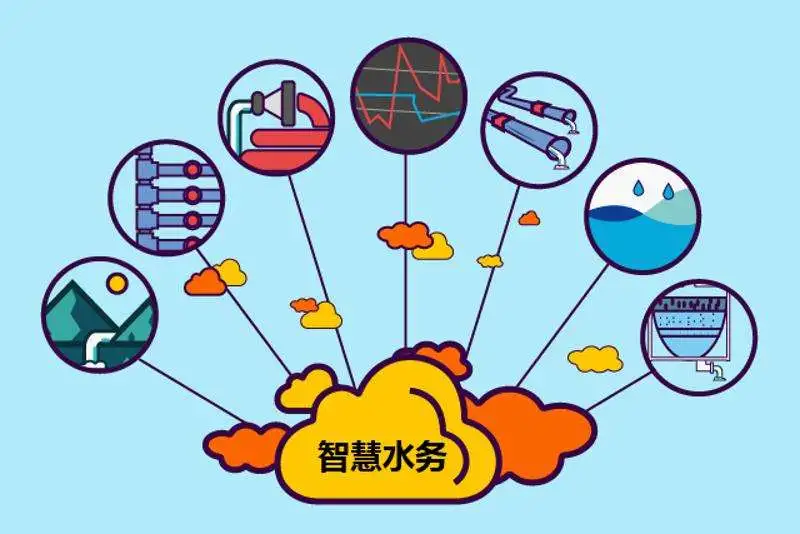
\includegraphics[width=.9\linewidth]{images/bg}
	\caption{\label{bg1}智慧水务}
\end{figure}

智慧水务是以先进的信息科技(应用水务物联网数据采集、大数据[l1]分析、模型仿真、移动化应用等)和先进的水领域专业技术为手段,以行业先进管理模式为标杆,以提升服务、运营能力、管理决策水平和绩效表现为目标的智慧化平台。更通俗一点来说就是利用物联网、大数据、云平台等技术手段实现更好的水务信息化建设。

在当前如火如荼的智慧城市建设中,智慧水务是其中重要的组成部分。欧卡智能\cite{orca}依托水面无人驾驶技术,打造系列水面服务机器人实现高效的水域运维管理,同时结合公司在AI算法部分水面无人驾驶技术和机电一体化部分的整机/功能模块打造能力的丰富经验推出了系列的产品与解决方案:欧卡聚焦智慧水务管理平台下,用标准化水面无人驾驶服务机器人的方式进行水域管理与维护的三大解决方案:

\begin{itemize}
	\item 水面清洁环卫与维护
	\item 水域数据收集与监测(水质、水深、水下地形)
	\item 水域安防巡检与排查(违法人员、活动、排污探测)
\end{itemize}

面向城市水域:湖泊,水库、内河;以及近海水域:港口、海岸线沿岸;逐步形成一套逐步形成一套从数据化监控、智能化维护到网格化预测的智慧水务整体解决方案, 帮助水务企业打通企业内部乃至行业上下游的水域治理全套链条,实现对水域从监管、运营、服务等业务环节的高效管理,从而为智慧城市建设增添助力。

本次暑期实践主要关注“水面清洁环卫与维护”相关的内容,在此只介绍此部分的解决方案以及目前存在的问题。

\section{水面清洁环卫与维护}
水域清洁现有解决方案主要包括人工清理和打捞船清理。

\begin{note}[人工清理]
	依靠人工清理的方式,即采用半舱式或甲板机动驳船,由环卫工人手持网兜站在甲板上直接把垃圾捞上来,这种传统的打捞方法劳动强度大、工作环境恶劣,人身安全没有保证,清理垃圾效率低,且一般的机械化打捞设备作业面小,不能到达滩涂、狭窄河边工作,无法彻底清除垃圾。如图\ref{bg2}所示。
\end{note}

\begin{figure}[h]
	\centering
	\begin{subfigure}[b]{0.45\textwidth}
		\centering
		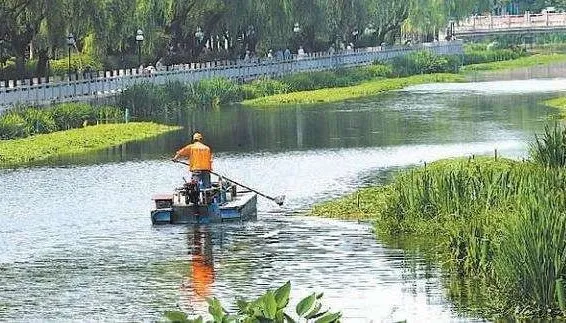
\includegraphics[width=.89\textwidth]{images/bg2}
		\caption{人工清理水域方式}
		\label{bg2}
	\end{subfigure}
	\hfill
	\begin{subfigure}[b]{0.46\textwidth}
		\centering
		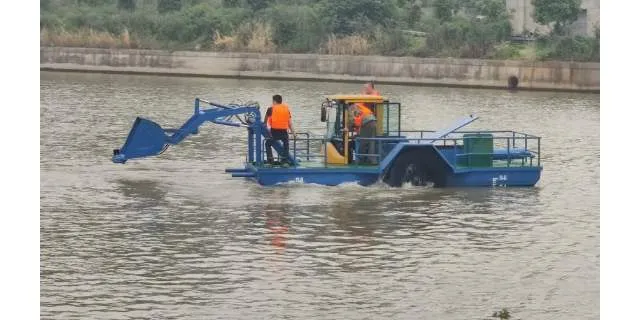
\includegraphics[width=\textwidth]{images/bg3}
		\caption{打捞船清理水域方式}
		\label{bg3}
	\end{subfigure}
\end{figure}

\begin{note}[打捞船清理]
	使用燃油驱动和人工驾驶的机械装置,但是体积较大,结构复杂且难以携带,不利于面积较小或形状复杂多变的城市河道、景观水池、饮用水库的垃圾清理,而且这些装置绝大多数使用燃油驱动,对清理水域会造成二次污染。如图\ref{bg3}所示。
\end{note}

考虑到以上问题,在湖泊、内河、水库的近海海域等水域生态区域,欧卡智能通过水面无人驾驶服务机器人平台,利用无线充电、高精度地图定位、垃圾识别等机电一体化技术,实现对水域漂浮垃圾的实时清理,不间断作业。通过水面无人驾驶技术,使得欧卡水面服务机器人在不需要遥控等人力干预下,即可自主完成清理作业,通过计算机、智能手持终端和物联网终端等设备,实现水质、垃圾等信息的实时查看、时空物联的远程精准控制。其相对于人工清理和大型水面清理装置的优势如图\ref{bg4}所示。

\begin{figure}[h]
	\centering
	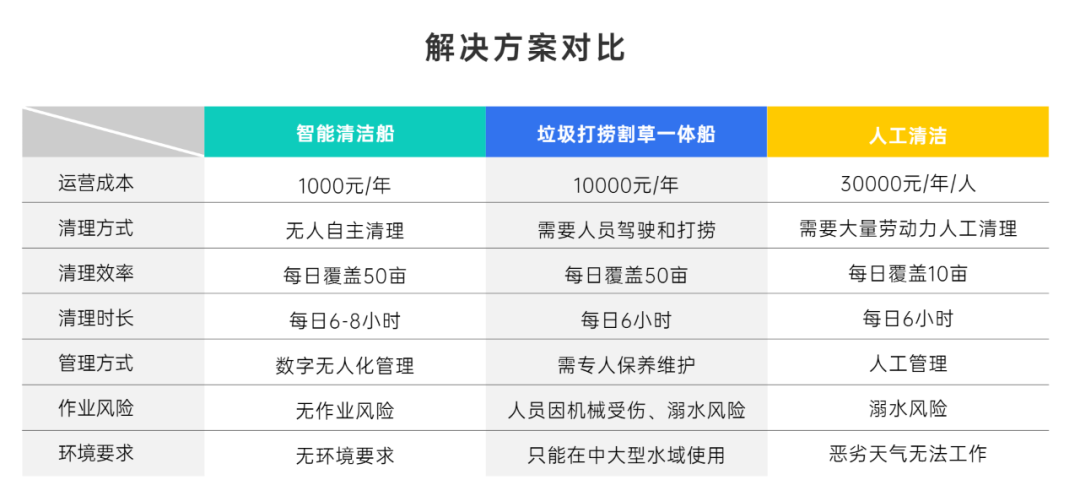
\includegraphics[width=.9\linewidth]{images/bg4}
	\caption{\label{bg4}智能清洁船与人工清理、大型水面清理船的对比}
\end{figure}

\section{现存问题与实践内容简述}
欧卡无人驾驶船已经在城市内河、景观湖泊、人工水库、近海港口等大部分环境下较为准确的执行清洁任务,而对于岸边的清洁仍然有一定的缺陷。由于在湖泊、内河等地会有很多垃圾聚集在岸边,因此能够近距离的贴着岸边清洁是一个非常重要的挑战。目前公司主要是利用雷达和GPS来检测和重建小船当前的环境来进行贴边清洁,但是由于GPS定位有一定的误差,尤其对于湖面上方有树丛遮挡的场景,GPS定位的误差会特别大,这也就导致了不能近距离的贴边带来的清洁效果不佳。

本次实践主要在计算机视觉的角度考虑,利用船头放置的摄像头拍摄当前场景,并结合图像语义分割等技术得到水岸线在摄像头视野中的位置,再利用逆投影的方式得到水岸线各个位置与摄像头之间的距离。实践相关代码已上传\url{https://github.com/luoyt14/orch_intern},主要内容包括如下两方面:
\begin{itemize}
	\item 基于计算机视觉的水岸线检测算法:包括deeplabv3plus\cite{chen2018encoderdecoder}、SETR\cite{zheng2021rethinking}、Segformer\cite{xie2021segformer}等基于图像语义分割的算法,以及Lane Detection\cite{qin2020ultra}的算法;
	\item 逆投影测距算法:一般来说,测距需要双目摄像头或者深度摄像头,单目无法测距,但是由于我们只需要水面上水岸线的点到摄像头的距离,拥有这些点都在同一个平面上的先验条件,使得单目相机测距成为可能。
\end{itemize}


\chapter{基于计算机视觉的水岸线检测算法}
本章介绍实践中使用的基于计算机视觉的水岸线检测算法,主要包括两个方面:
\begin{introduction}
	\item 基于图像语义分割的水岸线检测算法
	\item 基于lane detection的水岸线检测算法
\end{introduction}

\section{基于图像语义分割的水岸线检测算法}
本次实践中主要采用Deeplabv3plus、SETR、Segformer三种方法对船载摄像头拍摄到的图像进行分割,Deeplabv3plus是一种经典的基于encoder-decoder结构和CNN网络的语义分割算法,SETR是CVPR2021提出的基于vision transformer\cite{dosovitskiy2021image}结构的语义分割算法,Segformer是最近刚提出的一种基于Hierarchical Transformer Encoder和纯MLP decoder的语义分割算法,具体细节以及实验结果在后文给出。

\subsection{Deeplabv3plus}

\begin{figure}[h]
	\centering
	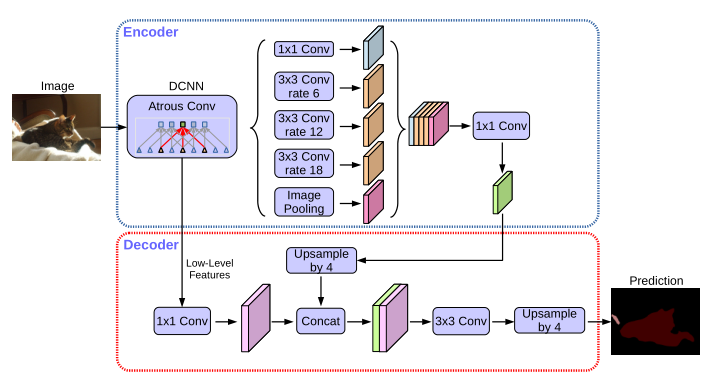
\includegraphics[width=.9\linewidth]{images/deeplabv3plus}
	\caption{\label{deeplabv3plus}DeepLabv3plus网络结构示意图}
\end{figure}

Deeplabv3plus\cite{chen2018encoderdecoder}采用Encoder-Decoder的架构,如图\ref{deeplabv3plus}所示,Encoder部分,实际上就是DeepLabV3\cite{chen2017rethinking}网络。首先选一个低层级的feature用$1\times 1$的卷积进行通道压缩(原本为256通道,或者512通道),目的是减少低层级的比重。由于编码器得到的feature具有更丰富的信息,所以编码器的feature有更高的比重,这样做有利于训练。对于Decoder部分,直接将编码器的输出上采样4倍,使其分辨率和低层级的feature一致。将两种feature连接后,再进行一次$3\times 3$的卷积(细化作用),然后再次上采样就得到了像素级的预测。

\begin{figure}[h]
	\centering
	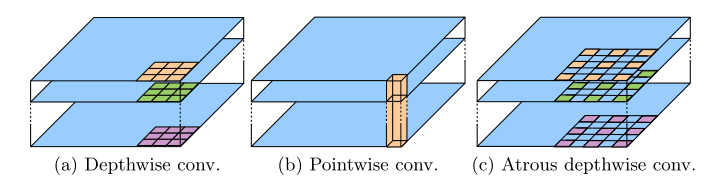
\includegraphics[width=.9\linewidth]{images/deeplabv3plus-2}
	\caption{\label{deeplabv3plus2}Depthwise卷积、Pointwise卷积以及空洞卷积示意图}
\end{figure}

其次网络中还用到了空洞卷积、可分离卷积来减小运算量,如图\ref{deeplabv3plus2}所示,可分离卷积是将传统的卷积分解成Depthwise conv和Pointwise conv来减小计算量的,在Deeplabv3plus中,将空洞卷积用于Depthwise conv中,在保持Deeplabv3中感受野的同时,减小了运算量。对于二维输入$x$,卷积核权重为$w$,空洞卷积系数为$r$的位置$i$处的输出$y$可计算如下:
\begin{equation}
	y[i]=\sum_k x[i+r\cdot k]w[k]
\end{equation}

训练使用的Loss函数为交叉熵损失函数,计算如下:
\begin{equation}
	\label{ce}
	L=-\sum_h^H\sum_w^W\sum_c^CY_{h,w,c}\log P_{h,w,c}
\end{equation}
其中$P\in\mathbb{R}^{H\times W\times C}$是网络的输出,$Y\in\mathbb{R}^{H\times W\times C}$是图像的label经过one-hot编码之后的张量,$H$是图像的高,$W$是图像的宽,$C$是图像语义分割的类别数。

\subsection{SETR}
对语义分割而言,上下文(context)信息是提升性能最关键的因素,而感受野(respect-field)则大致决定了网络能够利用到多少的信息。通常,在编码器中,我们会在下采样的过程中逐层的降低空间分辨率,以减少计算资源的消耗同时有效的扩大了网络的感受野。然而,相关研究表明,网络的实际感受野远小于其理论感受野,过多的下采样操作会导致小目标的细节信息被严重损失甚至完全丢失。因此,如何既能够抽取全局的语义信息,又能尽量不损失分辨率,一直是语义分割的难点。传统基于CNN的语义分割框架从空洞卷积、注意力机制的方向进行优化,在一定程度上提升了语义分割的性能。

近几年来,Transformer\cite{vaswani2017attention}和self-attention在自然语言处理领域取得了很好的成就,最近,也有很多人将Transformer用于图像识别领域,例如ViT\cite{dosovitskiy2021image}、DeiT\cite{touvron2020deit}等。由于Transformer的一个特性便是能够保持输入和输出的空间分辨率不变,同时还能够有效的捕获全局的上下文信息,可以很好的解决语义分割面临的问题。因此SETR采用Transformer作为Encoder来抽取全局的语义信息(整个过程不损失image分辨率),代替传统FCN的编码部分,从序列-序列学习的角度,为语义分割问题提供了一种新的视角。

\begin{figure}[h]
	\centering
	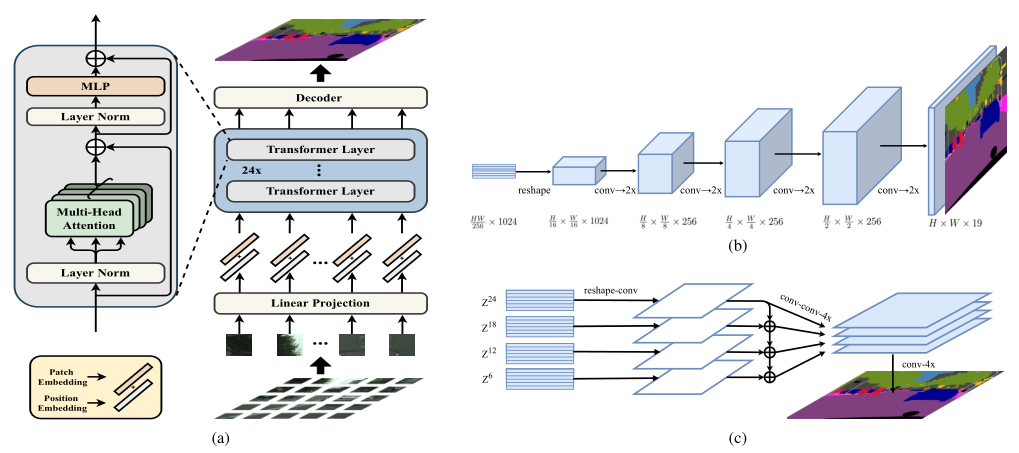
\includegraphics[width=.9\linewidth]{images/setr1}
	\caption{SETR示意图:(a)将图片切分成固定大小的patches,然后使用Linearly embed和位置编码,然后将其输入标准的Transformer结构中得到编码后的特征,为了能够进行逐像素的分割,使用了两种不同的解码器,(b)基于逐次上采样的解码器(将此种算法称为SETR-PUP),(c)基于多层特征融合的解码器(称为SETR-MLA)}
	\label{setr}
\end{figure}

\begin{note}[图像转换为序列数据输入]
	SETR的网络结构如图\ref{setr}所示,假设输入图片$x\in\mathbb{R}^{H\times W\times 3}$,按照$16\times16$的大小切分成$\frac{H}{16}\times\frac{W}{16}$个patches,对每一个patch $p\in\mathbb{R}^{16\times16\times3}$,使用一个线性映射函数$f:p\rightarrow e\in\mathbb{R}^C$得到1D的embedding向量。由于Transformer是无序的,因此学习了一个特定的位置映射$p_i$来表征图像中每个patch的位置信息,最后将$p_i$和$e_i$相加得到Transformer的输入序列数据$E=\{e_1+p_1,e_2+p_2,\dots,e_L+p_L\}\in \mathbb{R}^{L\times C}$,在SETR中$L=\frac{HW}{256}$。
\end{note}

\begin{note}[Transformer编码器]
	包括$L_e$层多头自注意力模块(Multi-head Self-Attention, MSA)和多层感知机模块(Multi-Layer Perceptron, MLP),对于每一层$l$,当前层的输入为上一层的输出为$Z^{l-1}\in \mathbb{R}^{L\times C}$(第一层的输入即为上一步得到的序列数据$E$),首先计算得到Transformer Layer输入的三元组(query,key,value):
	\begin{equation}
		\text{query}=Z^{l-1}W_Q,\quad \text{key}=Z^{l-1}W_K,\quad \text{value}=Z^{l-1}W_V
	\end{equation}
	其中$W_Q,W_K,W_V\in\mathbb{R}^{C\times d}$是三个线性层的参数,$d$是三元组(query,key,value)的维度。然后可以计算自注意力(self-attention,SA)如下:
	\begin{equation}
		SA(Z^{l-1})=Z^{l-1}+\text{softmax}(\frac{Z^{l-1}W_Q(Z^{l-1}W_K)^T}{\sqrt{d}})(Z^{l-1}W_V)
	\end{equation}
	MSA是将$m$个独立的SA连接起来,通过一个线性层得到输出,$MSA(Z^{l-1})=[SA_1(Z^{l-1});SA_2(Z^{l-1});\cdots;SA_m(Z^{l-1})]W_O$,其中$W_O\in\mathbb{R}^{md\times C}$,实际应用中$d$一般设为$C/m$,然后将MSA的输出过一个带跳跃连接的MLP模块,得到本层的输出:
	\begin{equation}
		Z^l=MSA(Z^{l-1})+MLP(MSA(Z^{l-1}))\in\mathbb{R}^{L\times C}
	\end{equation}
	将各个Transformer层的输出记为$\{Z^1,Z^2,\cdots,Z^{L_e}\}$
\end{note}

\begin{note}[解码器]
	将编码器得到的特征向量映射到原本图像大小来进行像素级的分割,首先将编码器得到的特征向量进行reshape:$\frac{HW}{256}\times C\Longrightarrow\frac{H}{16}\times\frac{W}{16}\times C$,然后通过解码器恢复到$H\times W\times categories$,本文主要有三种解码器设计:
	\begin{itemize}
		\item \textbf{Naive upsampling}:首先通过$1\times 1$的卷积将最后一层Transformer层的输出$Z^{L_e}$的维度映射为分割类别数(例如cityscapes 19类),然后通过双线性插值(大小$\times 16$)直接恢复到原图大小,此种算法简称为SETR-Naive;
		\item \textbf{Progressive UPsampling (PUP)}:如图\ref{setr}(b)所示,每次上采样到2倍大小,上采样4次得到原图大小,简称为SETR-PUP;
		\item \textbf{Multi-Level feature Aggregation (MLA)}:如图\ref{setr}(c)所示,将不同Transformer层的特征拿出来,首先reshape到$\frac{H}{16}\times\frac{W}{16}\times C$然后通过3个卷积层$1\times1, 3\times3, 3\times3$,在第一个和第三个卷积层将$C$缩减到原来的一半。然后将得到向量上采样4倍并且从上到下将各高层的向量逐元素相加到低层,再通过一个$3\times3$的卷积操作,然后将不同层得到的向量堆叠,最后双线性插值上采样4倍得到原图大小的解码输出,简称为SETR-MLA。
	\end{itemize}
\end{note}

训练使用的Loss函数依然是交叉熵损失函数\eqref{ce},除此之外,还使用了PSPNet\cite{zhao2017pyramid}中提到的辅助损失(Auxiliary loss)加速训练。

\subsection{Segformer}
虽然SETR已经有了足够好的效果,但仍然有一定的缺点:
\begin{itemize}
	\item 由于其使用ViT作为Encoder,参数量巨大,不太适用于直接部署到船载摄像头;
	\item ViT是柱状结构,全程只能输出固定分辨率的feature map,比如1/16,这么低的分辨率对于语义分割不太友好,尤其是对轮廓等细节要求比较精细的场景;
	\item ViT的柱状结构意味着一旦增大输入图片或者缩小patch大小,计算量都会成平方级提高,对显存的负担非常大;
	\item ViT用的是固定分辨率的positional embedding,但是语义分割在测试的时候往往图片的分辨率不是固定的,这时要么对positional embedding做双线性插值,这会损害性能,要么做固定分辨率的滑动窗口测试,这样效率很低而且很不灵活。
\end{itemize}

\begin{figure}[h]
	\centering
	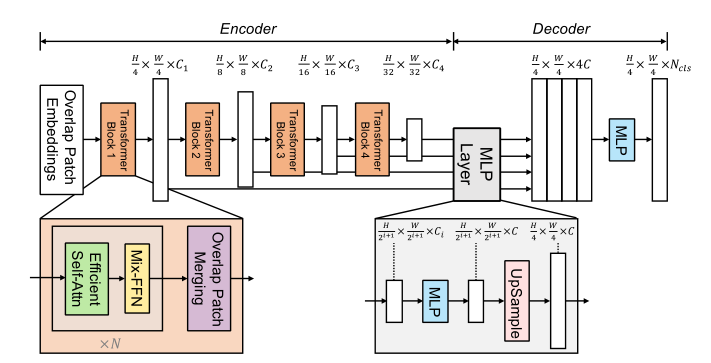
\includegraphics[width=.85\linewidth]{images/segformer}
	\caption{Segformer示意图。主要包括两个模块,1.层次化的Transformer编码器来提取粗细粒度的特征;2.简单轻量级的MLP解码器融合不同层次的特征并预测语义分割mask}
	\label{segformer}
\end{figure}

Segformer\cite{xie2021segformer}考虑到以上问题,重新设计了适用于语义分割的Transformer Encoder,并且仅使用简单轻量级的MLP作为Decoder,在不损失性能的前提下,极大的减小了模型的参数量大小,其网络结构如图\ref{segformer}所示。

\begin{note}[Hierarchical Transformer Encoder]
	主要包括如下几方面的改进:
	\begin{itemize}
		\item 之前ViT和PVT做patch embedding时,每个patch是独立的,这里对patch设计成有overlap的,这样可以保证局部连续性;
		\item 更高效的自注意力计算方法:原始的Attention计算方法为
		\begin{equation}
			Attention(Q,K,V)=Softmax(\frac{QK^T}{\sqrt{d_{head}}})V
		\end{equation}
		复杂度为$O(N^2)$。在此利用\cite{wang2021pyramid}中的方法进行以比例$R$进行维度缩减:
		\begin{equation}\begin{aligned}
			\hat{K}&=Reshape(\frac{N}{R},C\cdot R)(K) \\
			K&=Linear(C\cdot R,C)(\hat{K})
		\end{aligned}\end{equation}
		由此得到新的$K\in\mathbb{R}^{\frac{N}{R}\times C}$,自注意力计算复杂度缩减到$O(\frac{N^2}{R})$
		\item 彻底去掉了Positional Embedding,取而代之的是Mix FFN,即在feed forward network中引入3x3 deepwise conv传递位置信息,计算如下:
		\begin{equation}
			x_{out}=MLP(GELU(Conv_{3\times3}(MLP(x_{in}))))+x_{in}
		\end{equation}
	\end{itemize}
\end{note}

\begin{figure}[t]
	\centering
	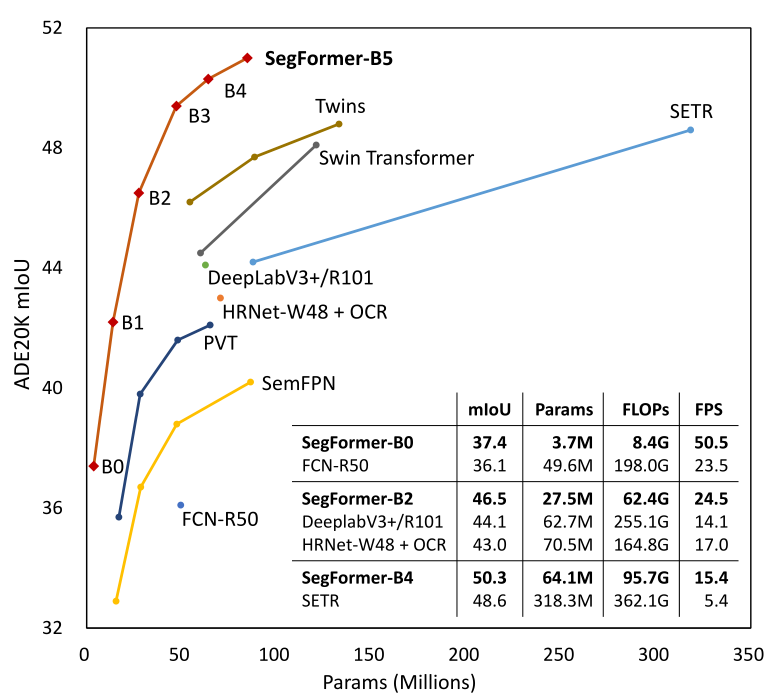
\includegraphics[width=.7\linewidth]{images/segformer2}
	\caption{Segformer B0-B5与其他算法在ADE20k\cite{zhou2017scene}上的性能对比,横坐标表示参数量,纵坐标表示mIoU}
	\label{segformer2}
\end{figure}

\begin{note}[Lightweight All-MLP Decoder]
	首先将MiT编码器不同层的特征$F_i\in\mathbb{R}^{\frac{H}{2^{i+1}}\times\frac{W}{2^{i+1}}\times C_i}(i=1,2,3,4)$通过一个MLP层统一维度,然后上采样到原图$1/4$大小并concatenate起来,然后再通过一个MLP层融合特征$F$,最后再使用一个MLP层将融合后的特征预测分辨率为$\frac{H}{4}\times\frac{W}{4}\times N_{cls}$分割mask,计算如下:
	\begin{equation}
		\begin{aligned}
			&\hat{F}_i=Linear(C_i,C)(F_i),\forall i \\
			&\hat{F}_i=Upsample(\frac{H}{4}\times\frac{W}{4})(\hat{F}_i),\forall i \\
			&F=Linear(4C,C)(Concat(\hat{F}_i)),\forall i \\
			&M=Linear(C,N_{cls})(F)
		\end{aligned}
	\end{equation}
\end{note}

训练使用的Loss函数依然是交叉熵损失函数\eqref{ce}。针对不同的overlap、Transformer参数,有Segformer B0-B5五种模型,B0最快、参数量最小,B5性能最好但是参数量较大,但是都比SETR参数量小很多,如图\ref{segformer2}所示。

\subsection{实验结果对比}
本小节将以上提到的3种算法在水面数据集上进行对比,使用python语言以及pytorch框架进行编写,在Nvidia RTX 3090显卡上进行实验,考虑到参数量与计算复杂度的问题,Deeplabv3plus使用了ResNet18\cite{he2016deep}作为backbone,Deeplabv3plus和SETR使用pytorch 1.9.0+cuda 11.1+mmcv\cite{mmcv} 1.3.9+mmsegmentation\cite{mmseg2020} 0.15.0环境进行实验,Segformer使用pytorch 1.8.0+cuda 11.1+mmcv\cite{mmcv} 1.2.7+mmsegmentation\cite{mmseg2020} 0.11.0环境进行实验。SETR使用了SETR-PUP用于实验,Segformer使用了Segformer-B5用于实验。训练数据使用公司已经发布的数据集USVInland Dataset\cite{9381638},分别在USVInland Dataset测试集以及使用小船采集的数据集上进行测试。

\begin{note}[训练集]
	是在不同的城市内河、景观湖泊、人工水库、近海港口等采集并进行了像素级的标记,只包括水和非水两个类别,如图\ref{train}所示,标记图中红色的表示水面,黑色的表示非水面的部分。在实际训练中选择了1297张图片进行训练,图像包含有$1280\times640$和$640\times 320$两种类型的分辨率,在实际训练中,我们将图像resize到$512\times 512$进行训练。
\end{note}

\begin{figure*}[!htp]
	\centering
	\begin{tabular}{cc}
		\rotatebox[x=4pt,y=15pt]{90}{原图} &  	
		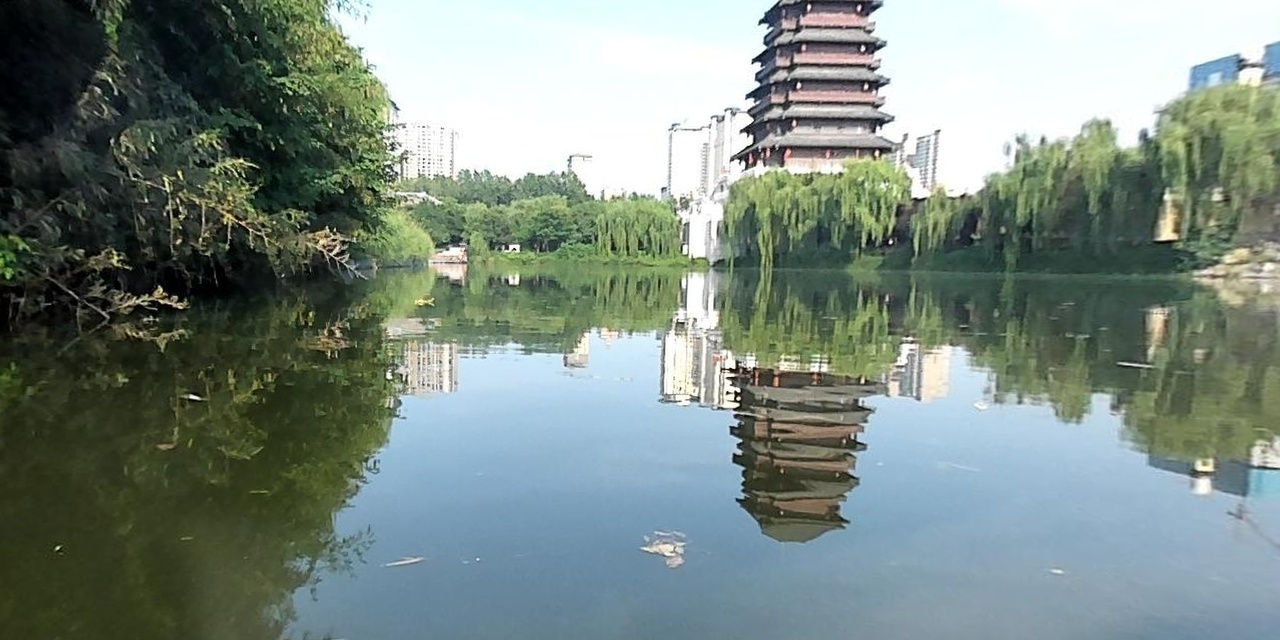
\includegraphics[width=0.23\linewidth]{results/train1}
		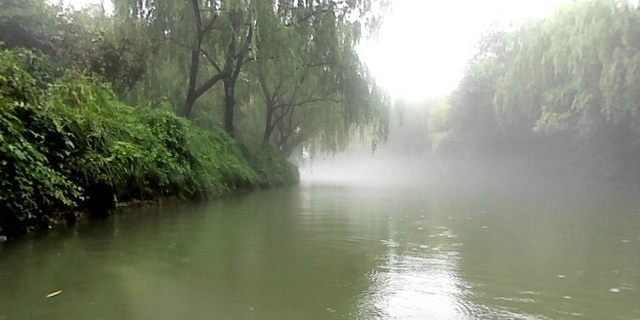
\includegraphics[width=0.23\linewidth]{results/train2}
		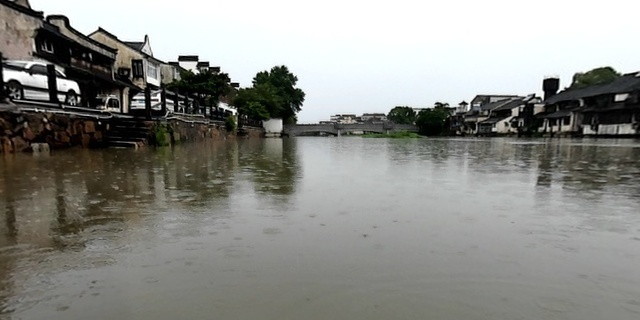
\includegraphics[width=0.23\linewidth]{results/train3}
		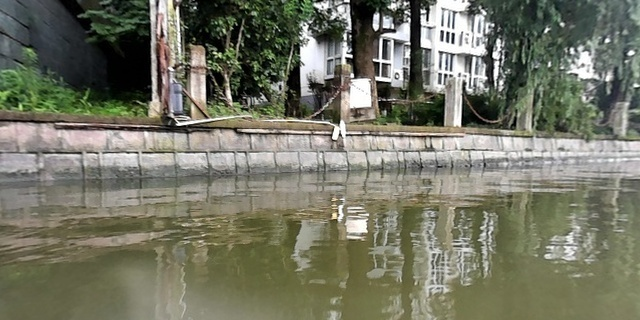
\includegraphics[width=0.23\linewidth]{results/train4}\\
		\rotatebox[x=2pt,y=38pt]{90}{GT} &  	
		\begin{subfigure}[b]{0.23\linewidth}
			\centering
\includegraphics[width=\linewidth]{results/train1gt}
			\caption{\label{fig:a}}
		\end{subfigure}
		\begin{subfigure}[b]{0.23\linewidth}
			\centering
\includegraphics[width=\linewidth]{results/train2gt}\caption{\label{fig:b}}
		\end{subfigure}
		\begin{subfigure}[b]{0.23\linewidth}
			\centering
\includegraphics[width=\linewidth]{results/train3gt}\caption{\label{fig:c}}
		\end{subfigure}
		\begin{subfigure}[b]{0.23\linewidth}
			\centering
\includegraphics[width=\linewidth]{results/train4gt}\caption{\label{fig:d}}
		\end{subfigure}
	\end{tabular}
	\caption{训练集数据示例图,第一行为原图,第二行为语义分割标记图(GT)}
	\label{train}
\end{figure*}

\begin{note}[USVInland Dataset上进行测试与评估]
	首先使用USVInland Dataset上剩下的数据作为测试集进行测试,并且采用mIoU来对3种不同的算法进行评估,IoU的计算如下:
	\[
		IoU=\frac{target\cap prediction}{target\cup prediction}
	\]
	即每个类别预测区域和真实区域的交集与并集的比值,mIoU为每个类别IoU的平均值。对于语义分割而言,mIoU越大说明分割效果越好,三种算法mIoU的对比如表\ref{res1}所示,可以看出水面分割这个任务中,Segformer的效果最好,但其实三种算法的精度都很高,基本都能正确的分割。可视化对比效果如图\ref{test1}所示,可以看出三种算法的分割效果都非常好,边缘也非常的整齐。
\end{note}

\begin{table}[h]
	\centering
	\caption{Deeplabv3plus, SETR, Segformer三种算法在USVInland Dataset上mIoU的对比}
	\label{res1}
	\begin{tabular}{cccc}
		\toprule
		算法 & deeplabv3plus & SETR & Segformer \\
		\midrule
		mIoU & 99.34 & 98.83 & \textbf{99.39} \\
		\bottomrule
	\end{tabular}
\end{table}

\begin{figure*}[!htp]
	\centering
	\begin{tabular}{cc}
		\rotatebox[x=4pt,y=15pt]{90}{原图} &  	
		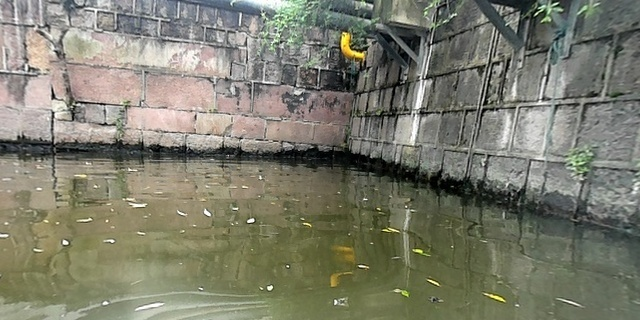
\includegraphics[width=0.23\linewidth]{results/test1}
		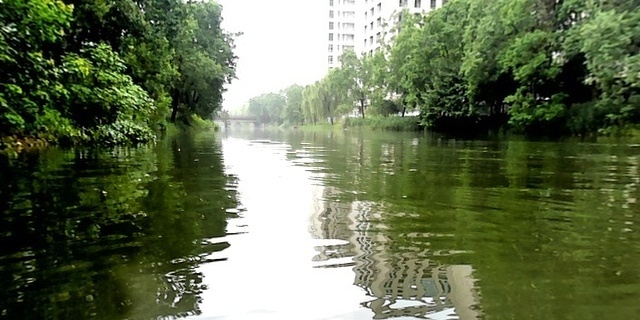
\includegraphics[width=0.23\linewidth]{results/test2}
		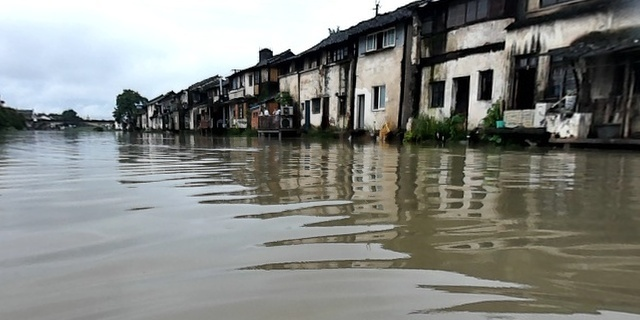
\includegraphics[width=0.23\linewidth]{results/test3}
		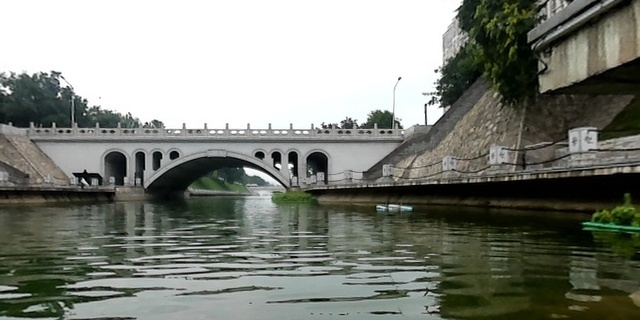
\includegraphics[width=0.23\linewidth]{results/test4}\\
		\rotatebox[x=4pt,y=26pt]{90}{GT} &  	
		
\includegraphics[width=0.23\linewidth]{results/test1gt}
		
\includegraphics[width=0.23\linewidth]{results/test2gt}
		
\includegraphics[width=0.23\linewidth]{results/test3gt}
		
\includegraphics[width=0.23\linewidth]{results/test4gt}\\
		\rotatebox[x=4pt,y=12pt]{90}{DeepLab} &  	
		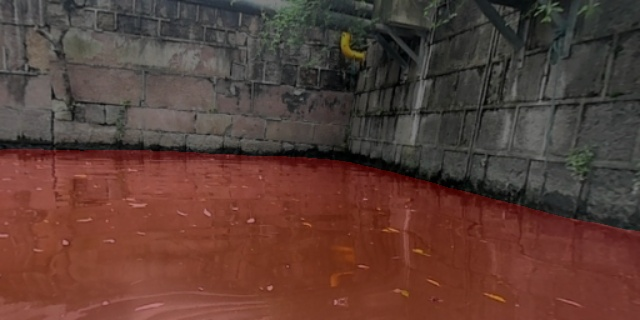
\includegraphics[width=0.23\linewidth]{results/test1deeplab}
		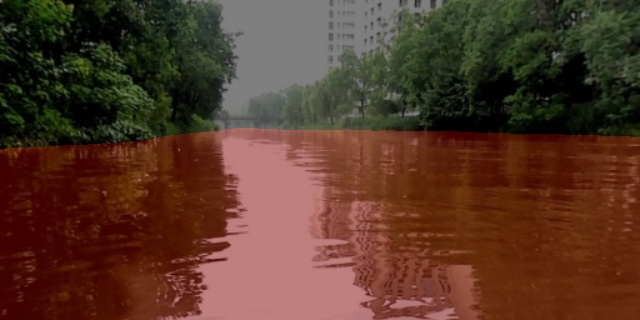
\includegraphics[width=0.23\linewidth]{results/test2deeplab}
		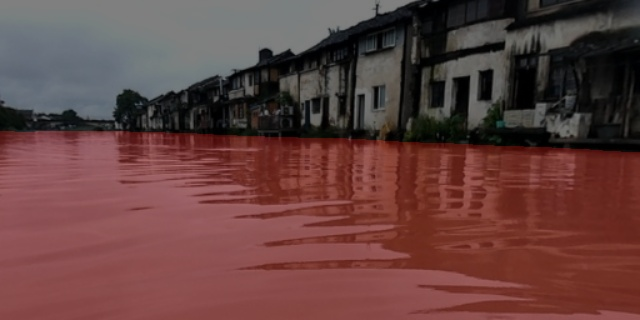
\includegraphics[width=0.23\linewidth]{results/test3deeplab}
		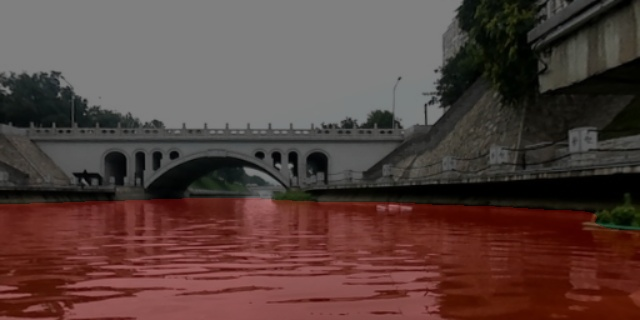
\includegraphics[width=0.23\linewidth]{results/test4deeplab}\\
		\rotatebox[x=4pt,y=15pt]{90}{SETR} &  	
		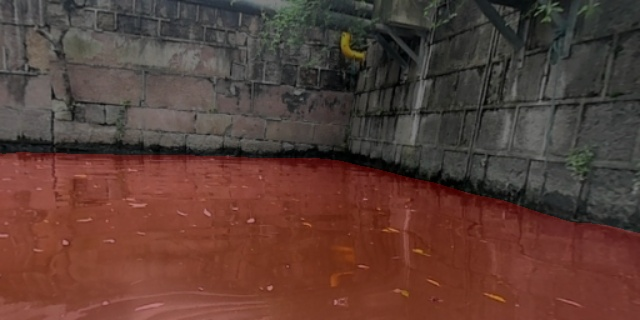
\includegraphics[width=0.23\linewidth]{results/test1setr}
		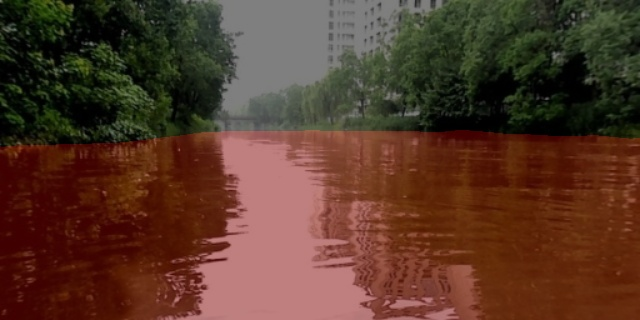
\includegraphics[width=0.23\linewidth]{results/test2setr}
		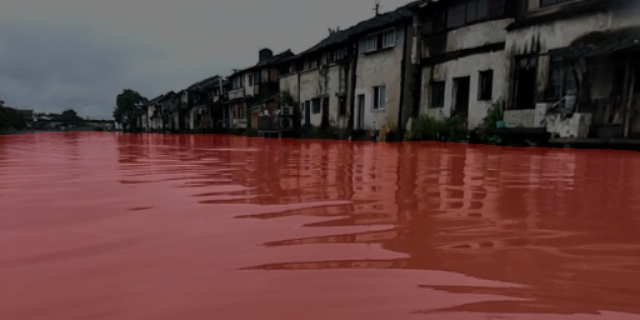
\includegraphics[width=0.23\linewidth]{results/test3setr}
		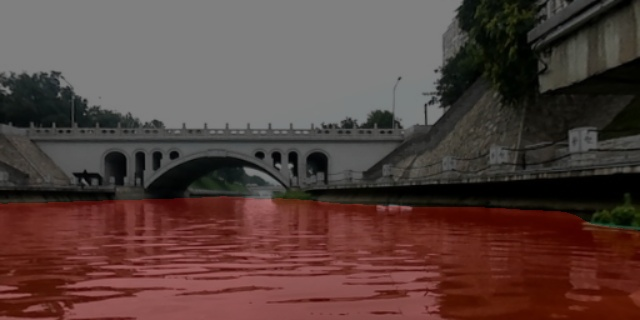
\includegraphics[width=0.23\linewidth]{results/test4setr}\\
		\rotatebox[x=2pt,y=25pt]{90}{Segformer} &  	
		\begin{subfigure}[b]{0.23\linewidth}
			\centering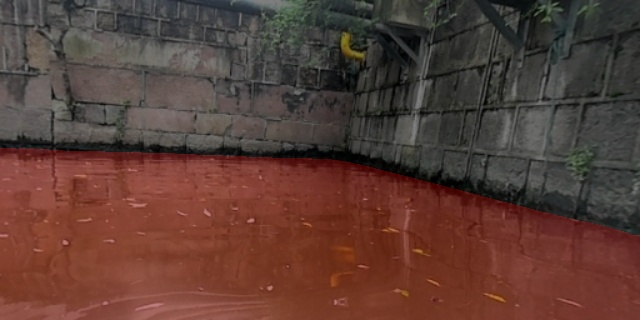
\includegraphics[width=\linewidth]{results/test1segformer}
			\caption{\label{fig:aa}}
		\end{subfigure}
		\begin{subfigure}[b]{0.23\linewidth}
			\centering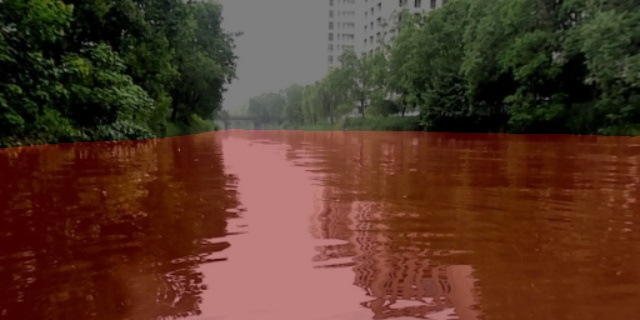
\includegraphics[width=\linewidth]{results/test2segformer}\caption{\label{fig:bb}}
		\end{subfigure}
		\begin{subfigure}[b]{0.23\linewidth}
			\centering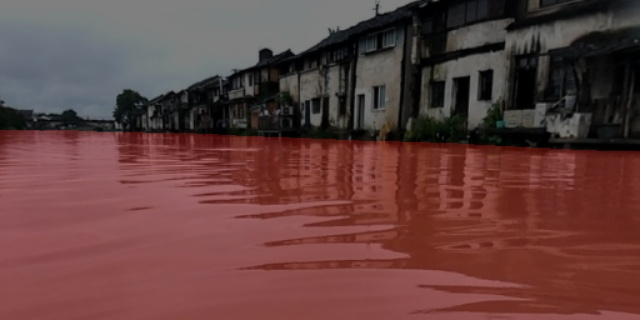
\includegraphics[width=\linewidth]{results/test3segformer}\caption{\label{fig:cc}}
		\end{subfigure}
		\begin{subfigure}[b]{0.23\linewidth}
			\centering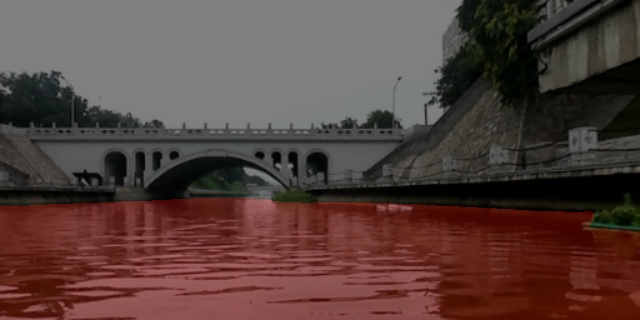
\includegraphics[width=\linewidth]{results/test4segformer}\caption{\label{fig:dd}}
		\end{subfigure}
	\end{tabular}
	\caption{USVInland Dataset测试集可视化对比图。第一行为测试集原图,第二行为语义分割标记图(GT),第三行为Deeplabv3plus算法的预测图,第四行为SETR算法的预测图,第五行为Segformer算法的预测图}
	\label{test1}
\end{figure*}

\begin{note}[自己采集数据集上的测试]
	从USVInland Dataset上的测试结果来看分割效果非常好,但由于训练集和测试集具有一定的相似性,因此有可能会有过拟合的现象。在此我们使用小船采集了西安外事学院鱼化湖的数据来做进一步的测试,这一批新采集的图像分辨率均为$640\times 480$,与训练集数据都不同。如图\ref{test2}所示,从第4、5行的对比图中可以看出,三种算法在大部分场景分割效果都比较好。第1行对比图中,deeplabv3plus在最左侧区域有误差,SETR边缘不够光滑,Segformer效果更好;第2行图同样SETR不够光滑,Segformer和deeplabv3plus效果较好;第3行图,在摄像头部分被树叶遮挡时,deeplabv3plus将树叶也分割到了水面类别中,属于分类错误,SETR和Segformer都正确检测到了树叶,效果更好一些。综上所述,三种算法中Segformer表现更加鲁棒一些,是较好的一个算法。
\end{note}

\begin{figure}[h]
	\centering
	\begin{subfigure}[b]{0.23\linewidth}
		\centering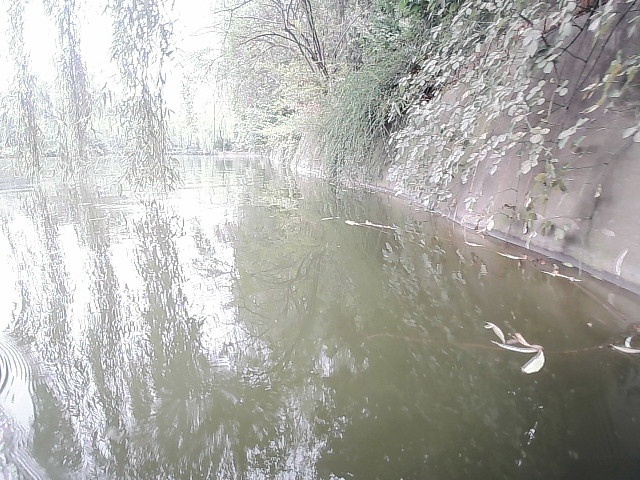
\includegraphics[width=\linewidth]{results2/test2}
	\end{subfigure}
	\begin{subfigure}[b]{0.23\linewidth}
		\centering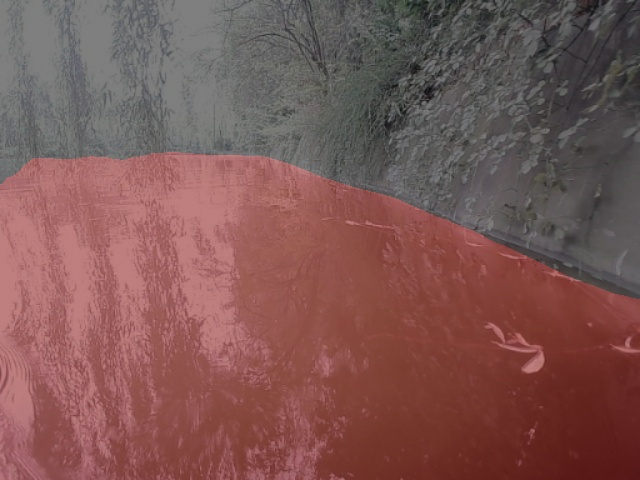
\includegraphics[width=\linewidth]{results2/test2deeplab}
	\end{subfigure}
	\begin{subfigure}[b]{0.23\linewidth}
		\centering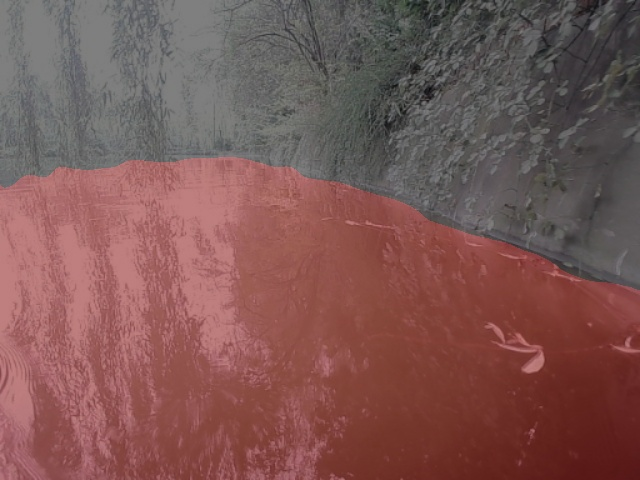
\includegraphics[width=\linewidth]{results2/test2setr}
	\end{subfigure}
	\begin{subfigure}[b]{0.23\linewidth}
		\centering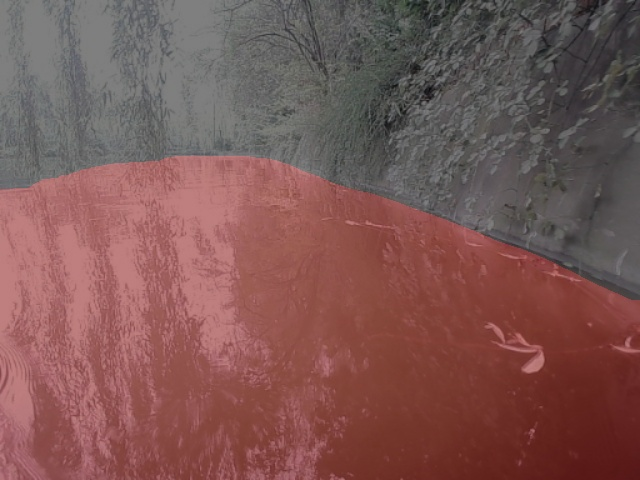
\includegraphics[width=\linewidth]{results2/test2segformer}
	\end{subfigure}\\
	\vspace{1mm}
	\begin{subfigure}[b]{0.23\linewidth}
		\centering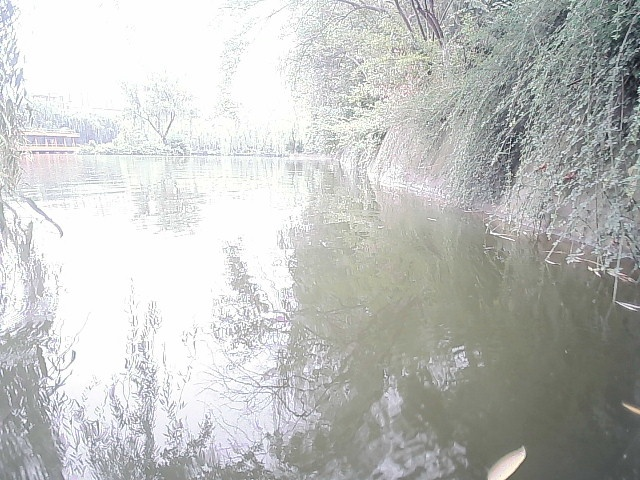
\includegraphics[width=\linewidth]{results2/test3}
	\end{subfigure}
	\begin{subfigure}[b]{0.23\linewidth}
		\centering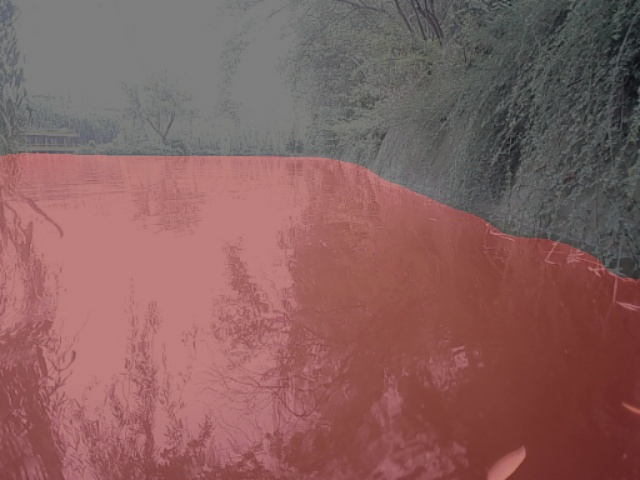
\includegraphics[width=\linewidth]{results2/test3deeplab}
	\end{subfigure}
	\begin{subfigure}[b]{0.23\linewidth}
		\centering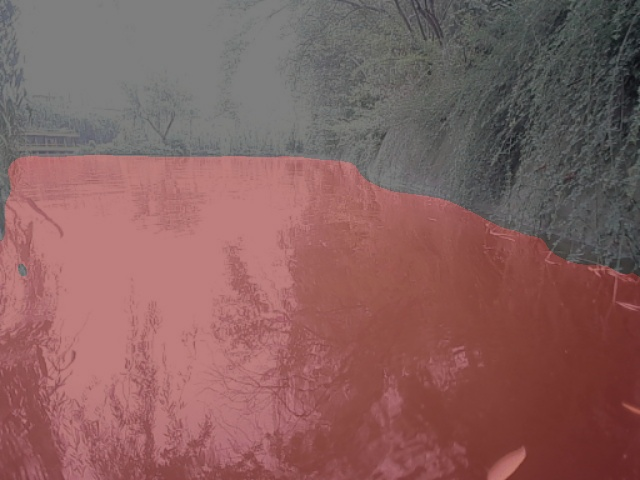
\includegraphics[width=\linewidth]{results2/test3setr}
	\end{subfigure}
	\begin{subfigure}[b]{0.23\linewidth}
		\centering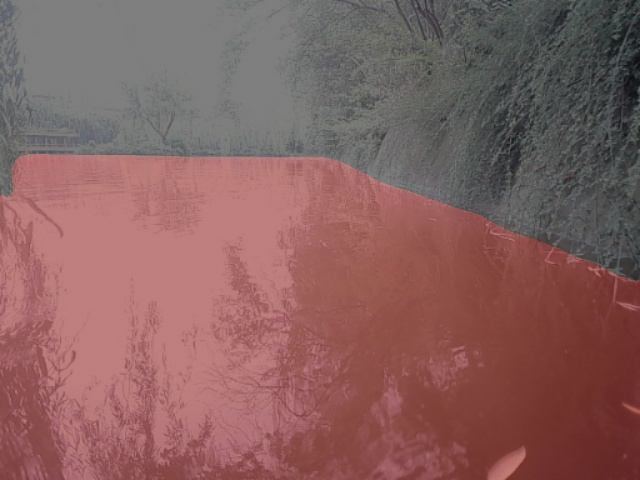
\includegraphics[width=\linewidth]{results2/test3segformer}
	\end{subfigure}\\
	\vspace{1mm}
	\begin{subfigure}[b]{0.23\linewidth}
		\centering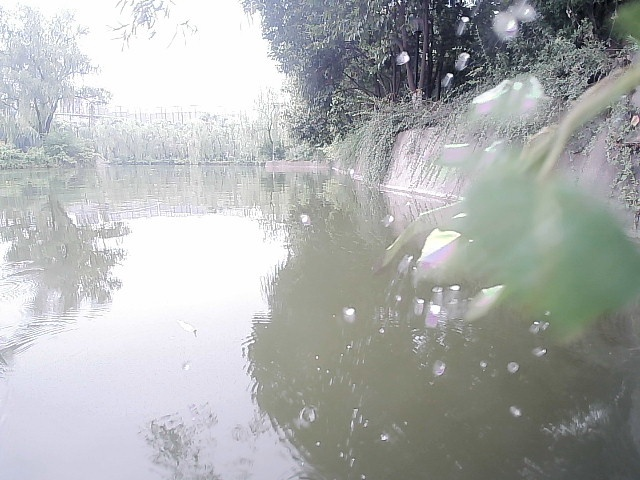
\includegraphics[width=\linewidth]{results2/test5}
	\end{subfigure}
	\begin{subfigure}[b]{0.23\linewidth}
		\centering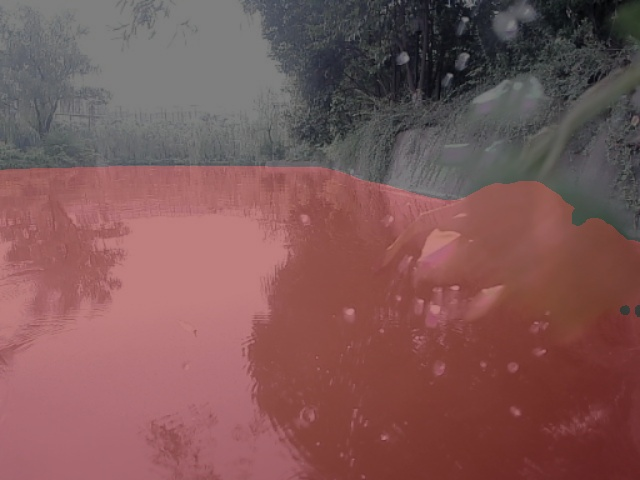
\includegraphics[width=\linewidth]{results2/test5deeplab}
	\end{subfigure}
	\begin{subfigure}[b]{0.23\linewidth}
		\centering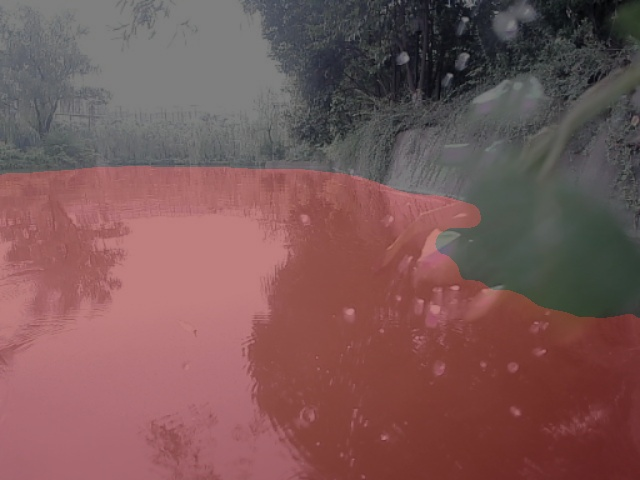
\includegraphics[width=\linewidth]{results2/test5setr}
	\end{subfigure}
	\begin{subfigure}[b]{0.23\linewidth}
		\centering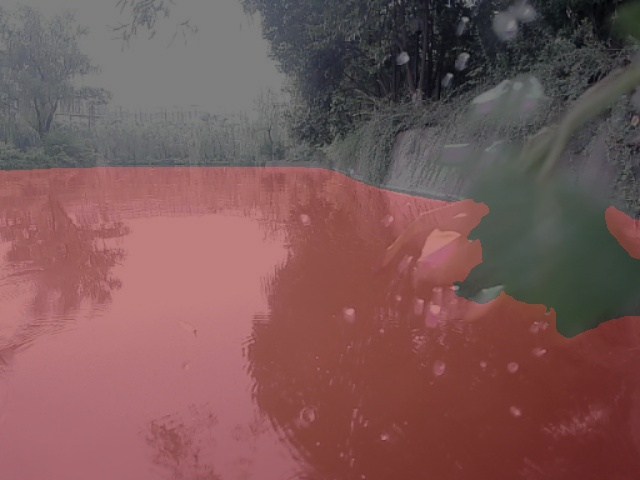
\includegraphics[width=\linewidth]{results2/test5segformer}
	\end{subfigure}\\
	\vspace{1mm}
	\begin{subfigure}[b]{0.23\linewidth}
		\centering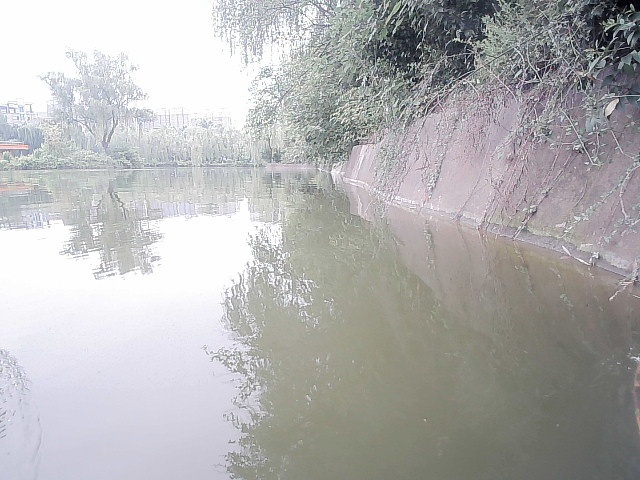
\includegraphics[width=\linewidth]{results2/test4}
	\end{subfigure}
	\begin{subfigure}[b]{0.23\linewidth}
		\centering\includegraphics[width=\linewidth]{results2/test4deeplab}
	\end{subfigure}
	\begin{subfigure}[b]{0.23\linewidth}
		\centering\includegraphics[width=\linewidth]{results2/test4setr}
	\end{subfigure}
	\begin{subfigure}[b]{0.23\linewidth}
		\centering\includegraphics[width=\linewidth]{results2/test4segformer}
	\end{subfigure}\\
	\vspace{1mm}
	\begin{subfigure}[b]{0.23\linewidth}
		\centering\includegraphics[width=\linewidth]{results2/test6}
		\caption{\label{fig:ori}原图}
	\end{subfigure}
	\begin{subfigure}[b]{0.23\linewidth}
		\centering\includegraphics[width=\linewidth]{results2/test6deeplab}\caption{\label{fig:deeplab}Deeplab分割图}
	\end{subfigure}
	\begin{subfigure}[b]{0.23\linewidth}
		\centering\includegraphics[width=\linewidth]{results2/test6setr}\caption{\label{fig:setr}SETR分割图}
	\end{subfigure}
	\begin{subfigure}[b]{0.23\linewidth}
		\centering\includegraphics[width=\linewidth]{results2/test6segformer}\caption{\label{fig:segformer}Segformer分割图}
	\end{subfigure}
	\caption{\label{test2}西安外事学院鱼化湖场景三种算法对比图}
\end{figure}


\section{基于lane detection的水岸线检测算法}
对于无人船贴边清洁而言,只需要检测到小船左侧或者右侧小范围内的岸边即可,使用语义分割算法进行逐像素分类浪费了大量的计算资源,对于清洁小船而言,降低计算复杂度与推理时间更为重要,在此我们将车道线检测算法Ultra Fast Structure-aware Deep Lane Detection\cite{qin2020ultra}加以改进用于我们的水岸线检测中。

\subsection{算法原理}
将车道线检测定义为寻找车道线在图像中某些行的位置的集合,即基于行方向上的位置选择、分类(row-based classification),如图\ref{lane1}所示,假设要检测一条车道线的图像大小为$H\times W$,对于分割问题,我们需要处理$H\times W$个分类问题。由于方案是行向选择,假设在$h$个行上做选择,只需要处理$h$个行上的分类问题,只不过每行上的分类问题是$W$维的。因此这样就把原来$H\times W$个分类问题简化为了只需要$h$个分类问题,而且由于在哪些行上进行定位是可以人为设定的,因此$h$的大小可以按需设置,但一般$h$都是远小于图像高度$H$的。

\begin{figure}[h]
	\centering
	\includegraphics[width=.95\linewidth]{images/lane1}
	\caption{基于行选择的车道线检测示意图}
	\label{lane1}
\end{figure}

算法整体结构图如图\ref{lane2}所示,Main branch用于训练和测试,Auxiliary branch只用于训练,在Auxiliary branch使用分割的交叉熵损失函数$L_{seg}$\eqref{ce}。考虑到连续性问题,每一行预测的位置也抛弃了传统的$Loc_{i,j}=\arg\max_k P_{i,j,k},k\in[1,w]$,而采用加权和的形式:
\begin{equation}
	\begin{aligned}
		&Prob_{i,j,:}=softmax(P_{i,j,1:w}) \\
		&Loc_{i,j}=\sum_{k=1}^wk\cdot Prob_{i,j,k}
	\end{aligned}
\end{equation}

在主分支使用三个损失函数(车道线数量为$C$,预测的概率为$P\in\mathbb{R}^{C\times h\times (w+1)}$,one-hot编码的真值为$T\in\mathbb{R}^{C\times h\times (w+1)}$,$(w+1)$主要是考虑到当前行可能没有车道线的情况):

\begin{itemize}
	\item 分类损失:对于选择的每一行,都是一个分类问题,同样使用交叉熵损失函数:
	\begin{equation}
		L_{cls}=\sum_{i=1}^{C}\sum_{j=1}^hL_{CE}(P_{i,j,:},T_{i,j,:})
	\end{equation}
	\item 连续性:考虑到车道线是连续的,因此使用一阶差分来定义连续性损失:
	\begin{equation}
		L_{sim}=\sum_{i=1}^{C}\sum_{j=1}^{h-1}||P_{i,j,:}-P_{i,j+1,:}||_1
	\end{equation}
	\item 线性:考虑到大部分车道线是直的,因此采用二阶差分来定义线性损失:
	\begin{equation}
		L_{shp}=\sum_{i=1}^{C}\sum_{j=1}^{h-2}||(Loc_{i,j,:}-Loc_{i,j+1,:})-(Loc_{i,j+1,:}-Loc_{i,j+2,:})||_1
	\end{equation}
\end{itemize}

最后总的损失通过三个损失函数加权得到,由于我们水岸线检测中不一定是直线,因此我们直接将二阶差分损失函数设置为0,总损失计算如下:
\begin{equation}
	L_{total}=L_{cls}+\alpha L_{sim}+0\cdot L_{shp}+\beta L_{seg}
\end{equation}

\begin{figure}[h]
	\centering
	\includegraphics[width=.95\linewidth]{images/lane2}
	\caption{lane detection算法结构图}
	\label{lane2}
\end{figure}

\subsection{数据标注}
由于此种算法与分割算法使用的数据集不一样,因此我们首先使用labelme\cite{labelme2016}标注了一批图像用于训练和测试,训练集共2424张图片,测试集共607张图片,训练集示例图像如图\ref{lane}所示。

\begin{figure*}[!htp]
	\centering
	\begin{tabular}{cc}
		\rotatebox[x=4pt,y=35pt]{90}{原图} &  	
		\includegraphics[width=0.23\linewidth]{lane/train1}
		\includegraphics[width=0.23\linewidth]{lane/train2}
		\includegraphics[width=0.23\linewidth]{lane/train3}
		\includegraphics[width=0.23\linewidth]{lane/train4}\\
		\rotatebox[x=2pt,y=58pt]{90}{GT} &  	
		\begin{subfigure}[b]{0.23\linewidth}
			\centering\includegraphics[width=\linewidth]{lane/train1gt}
			\caption{\label{lane:a}}
		\end{subfigure}
		\begin{subfigure}[b]{0.23\linewidth}
			\centering\includegraphics[width=\linewidth]{lane/train2gt}\caption{\label{lane:b}}
		\end{subfigure}
		\begin{subfigure}[b]{0.23\linewidth}
			\centering\includegraphics[width=\linewidth]{lane/train3gt}\caption{\label{lane:c}}
		\end{subfigure}
		\begin{subfigure}[b]{0.23\linewidth}
			\centering\includegraphics[width=\linewidth]{lane/train4gt}\caption{\label{lane:d}}
		\end{subfigure}
	\end{tabular}
	\caption{lane detection数据示例图,第一行为原图,第二行为水岸线标记图(GT)}
	\label{lane}
\end{figure*}

\subsection{实验结果}
此部分实验使用Nvidia RTX 1070显卡进行实验,使用pytorch 1.1.0+cuda 9.1环境进行实验,实验采用自己标注的数据作为训练集和测试集,可视化结果如图\ref{lane-res}所示,可以看出使用此算法能够很精确的检测到比较常规的岸边,但是对于特殊场景(例如:桥下-图\ref{lane-res}(d)),检测有一定的误差。

\begin{figure*}[!htp]
	\centering
	\begin{tabular}{cc}
		\rotatebox[x=4pt,y=35pt]{90}{原图} &  	
		\includegraphics[width=0.23\linewidth]{lane/test1}
		\includegraphics[width=0.23\linewidth]{lane/test2}
		\includegraphics[width=0.23\linewidth]{lane/test3}
		\includegraphics[width=0.23\linewidth]{lane/test4}\\
		\rotatebox[x=4pt,y=35pt]{90}{GT} &  	
		\includegraphics[width=0.23\linewidth]{lane/test1gt}
		\includegraphics[width=0.23\linewidth]{lane/test2gt}
		\includegraphics[width=0.23\linewidth]{lane/test3gt}
		\includegraphics[width=0.23\linewidth]{lane/test4gt}\\
		\rotatebox[x=2pt,y=58pt]{90}{预测结果} &  	
		\begin{subfigure}[b]{0.23\linewidth}
			\centering\includegraphics[width=\linewidth]{lane/test1res}
			\caption{\label{lane2:a}}
		\end{subfigure}
		\begin{subfigure}[b]{0.23\linewidth}
			\centering\includegraphics[width=\linewidth]{lane/test2res}\caption{\label{lane2:b}}
		\end{subfigure}
		\begin{subfigure}[b]{0.23\linewidth}
			\centering\includegraphics[width=\linewidth]{lane/test3res}\caption{\label{lane2:c}}
		\end{subfigure}
		\begin{subfigure}[b]{0.23\linewidth}
			\centering\includegraphics[width=\linewidth]{lane/test4res}\caption{\label{lane2:d}}
		\end{subfigure}
	\end{tabular}
	\caption{lane detection算法实验可视化结果图}
	\label{lane-res}
\end{figure*}

并且我们对比了三种基于语义分割的算法和此算法平均推理一张图所需要的时间如表\ref{res2}所示,可以看出lane detection的平均一张图的推理时间比其他三种基于语义分割的算法快10倍左右,在实际应用中可以更好的发挥作用。

\begin{table}[h]
	\centering
	\caption{Deeplabv3plus, SETR, Segformer三种基于语义分割的算法和lane detection算法平均推理一张图片所用时间对比}
	\label{res2}
	\begin{tabular}{ccccc}
		\toprule
		算法 & deeplabv3plus & SETR & Segformer & Lane Detection \\
		\midrule
		时间(s) & 0.03342 & 0.04954 & 0.06455 & \textbf{0.00337} \\
		\bottomrule
	\end{tabular}
\end{table}

\begin{note}[总结]
	在实际应用中使用lane detection的算法更快,但是其鲁棒性不太够,可能是由于数据量较少的原因。针对鲁棒性和精度而言,Segformer更好,可以利用Segformer算法去标记一部分数据,训练lane detection算法来获得更好的效果。
\end{note}

\chapter{逆投影测距算法}
在自动/辅助驾驶中,在前视摄像头拍摄的图像中,由于透视效应的存在,本来平行的事物,在图像中确实相交的。而逆投影(Inverse Perspective Mapping, IPM)变换就是消除这种透视效应,所以也叫逆透视。IPM将摄像头拍摄的图像进行转换成鸟瞰图,本质上是二维平面到二维平面的转换。通过图像上的一个点,可以估计其真实位置。本章主要考虑两种基于逆投影的测距算法:
\begin{introduction}
	\item Adaptive IPM
	\item 基于单应性矩阵的测距
\end{introduction}

\section{Adaptive IPM}
Adaptive IPM\cite{jeong2016adaptive}主要是利用相机成像原理和空间立体几何关系来推导出照片上水面上的点对应的真实距离。对于图像像素坐标来说,坐标原点一般是左上角,而对于相机而言,图像的坐标原点在中心,如图\ref{ordi}所示。

\begin{figure}[h]
	\centering
	\includegraphics[width=.65\linewidth]{images/camera}
	\caption{相机坐标系、像素坐标系与世界坐标系的关系}
	\label{ordi}
\end{figure}

根据几何关系,我们可以得到相机坐标系($\hat{\mathbf{r}},\hat{\mathbf{c}}$)与像素坐标系($\hat{\mathbf{u}},\hat{\mathbf{v}}$)的互化关系:
\begin{equation}
	\begin{aligned}
		&\mathbf{u}(\mathbf{c})=\frac{\mathbf{n}+1}{2}+\mathbf{K} \mathbf{c} \longleftrightarrow \mathbf{c}(\mathbf{u})=\frac{1}{\mathbf{K}}\left(\mathbf{u}-\frac{\mathbf{n}+1}{2}\right)\\
		&\mathbf{v}(\mathbf{r})=\frac{\mathbf{m}+1}{2}-\mathbf{K r} \longleftrightarrow \mathbf{r}(\mathbf{v})=\frac{1}{\mathbf{K}}\left(\frac{\mathbf{m}+1}{2}-\mathbf{v}\right)
	\end{aligned}
\end{equation}
其中$\mathbf{K}$是像素和米的变换比例(px/m)。然后绘制出相机投影的侧视图如图\ref{ceshi}所示,可以推导出图像上点对应实际位置与相机的垂直距离$\mathbf{X}$(从示意图中可以看出,这个距离只和图像的垂直像素距离$\mathbf{v}$有关):
\begin{align}
	&\mathbf{X}(\mathbf{v})=\mathbf{h} \cot \left(\theta_{0}-\theta(v)\right) \\
	&\theta(v)=\arctan \left(\frac{\mathbf{r}(\mathbf{v})}{\mathbf{f}_{\mathbf{r}}}\right) \\
	&\tan \left(\alpha_{r}\right)=\frac{\mathbf{r}_{t o p}}{\mathbf{f}_{\mathbf{r}}} \\
	&\mathbf{r}_{t o p}=\mathbf{r}(\mathbf{v}=1)=\frac{1}{\mathbf{K}} \frac{\mathbf{m}-1}{2} \\
	&\mathbf{f}_{\mathbf{r}}=\mathbf{r}_{t o p} \cot \left(\alpha_{r}\right)=\frac{\mathbf{m}-1}{\mathbf{2} \mathbf{K}} \cot \left(\alpha_{r}\right)
\end{align}
因此有:
\begin{equation}
\begin{aligned}
	\theta(\mathbf{v}) &=\arctan \left(\frac{\mathbf{r}(\mathbf{v})}{\mathbf{f}_{\mathrm{r}}}\right) \\
	&=\arctan \left(\left(1-2 \frac{\mathbf{v}-1}{\mathbf{m}-1}\right) \tan \left(\alpha_{r}\right)\right)
\end{aligned}
\end{equation}
\begin{equation}
\begin{aligned}
		\mathbf{X}(\mathbf{v}) &=\mathbf{h} \cot \left(\theta_{0}-\theta(v)\right) \\
		&=\mathbf{h} \frac{\tan \left(\theta_{0}\right) \tan (\theta(\mathbf{v}))+\mathbf{1}}{\tan \left(\theta_{0}\right)-\tan (\theta(\mathbf{v}))} \\
		&=\mathbf{h} \frac{\tan \left(\theta_{0}\right)\left(1-2 \frac{\mathbf{v}-1}{\mathrm{~m}-1}\right) \tan \left(\alpha_{r}\right)+\mathbf{1}}{\tan \left(\theta_{0}\right)-\left(1-2 \frac{\mathbf{v}-1}{\mathrm{~m}-1}\right) \tan \left(\alpha_{r}\right)}
\end{aligned}
\end{equation}

\begin{figure}[h]
	\centering
	\includegraphics[width=.75\linewidth]{images/ceshi}
	\caption{相机投影的侧视图}
	\label{ceshi}
\end{figure}

得到$\mathbf{X}(\mathbf{v})$之后,再看俯视图\ref{fushi},可以看出图像上点对应实际位置与相机的水平距离$\mathbf{Y}$与垂直像素距离$\mathbf{v}$和水平像素距离$\mathbf{u}$均有关系,根据相似三角形的性质有:
\begin{equation}
	\frac{\mathbf{Y}(\mathbf{u}, \mathbf{v})}{\mathbf{X}(\mathbf{v})}=-\frac{\mathbf{c}}{\mathbf{f}_{\mathrm{c}}}
\end{equation}

根据几何性质有如下关系:
\begin{align}
	&\tan \left(\alpha_{c}\right)=\frac{\mathbf{c}_{\text {right }}}{\mathbf{f}_{\mathbf{c}}} \\
	&\mathbf{c}_{r i g h t}=\mathbf{c}(\mathbf{u}=\mathbf{n})=\frac{1}{\mathbf{K}}\left(\frac{\mathbf{n}-1}{2}\right) \\
	&\mathbf{f}_{\mathrm{c}}=\frac{\mathbf{c}_{\text {right }}}{\tan \left(\alpha_{c}\right)}=\frac{\mathbf{n}-\mathbf{1}}{\mathbf{2 K} \tan \left(\alpha_{c}\right)}
\end{align}

因此可以得到:
\begin{equation}
	\begin{aligned}
		\mathbf{Y}(\mathbf{u}, \mathbf{v}) &=-\frac{\mathbf{1}}{\mathbf{K}}\left(\mathbf{u}-\frac{\mathbf{n}+\mathbf{1}}{\mathbf{2}}\right) \frac{\mathbf{2} \mathbf{K} \tan \left(\alpha_{c}\right)}{\mathbf{n}-\mathbf{1}} \mathbf{X}(\mathbf{v}) \\
		&=\left(\mathbf{1}-\mathbf{2} \frac{\mathbf{u}-\mathbf{1}}{\mathbf{n}-\mathbf{1}}\right) \tan \left(\alpha_{c}\right) \mathbf{X}(\mathbf{v})
	\end{aligned}
\end{equation}

\begin{figure}[h]
	\centering
	\includegraphics[width=.65\linewidth]{images/fushi}
	\caption{相机投影的俯视图}
	\label{fushi}
\end{figure}

这样便得到了静止状态下的图像上的点对应水面上实际位置距离摄像头的距离。但是当船行驶起来的时候,俯仰角会发生变化,即$\theta_{0}$会发生变化。如图\ref{ceshi2}所示,此时相当于原先的$\theta_{0}$变成了$\theta_{0}+\theta_p$,因此我们可以得到动态变化下的距离公式:

\begin{equation}
	\begin{aligned}
		\mathbf{X}\left(\mathbf{v}, \theta_{\mathbf{p}}\right) &=\mathbf{h} \frac{\tan \left(\theta_{0}+\theta_{p}\right)\left(1-2 \frac{\mathbf{v}-1}{\mathbf{m}-\mathbf{1}}\right) \tan \left(\alpha_{r}\right)+1}{\tan \left(\theta_{0}+\theta_{p}\right)-\left(1-2 \frac{\mathbf{v}-1}{\mathbf{m}-1}\right) \tan \left(\alpha_{r}\right)} \\
		\mathbf{Y}\left(\mathbf{u}, \mathbf{v}, \theta_{\mathbf{p}}\right) &=\left(1-2 \frac{\mathbf{u}-1}{\mathbf{n}-1}\right) \tan \left(\alpha_{c}\right) \mathbf{X}\left(\mathbf{v}, \theta_{\mathbf{p}}\right)
	\end{aligned}
\end{equation}

\begin{figure}[h]
	\centering
	\includegraphics[width=.75\linewidth]{images/ceshi2}
	\caption{俯仰角变化的相机投影的侧视图}
	\label{ceshi2}
\end{figure}

从示意图中可以看出,此场景只能计算出摄像头所在高度水平线以下的部分,而对于摄像头平视、仰视的场景无法很好的处理,因此在小船上不太适用,在实际测试中也证实了这一点,3m以内范围的误差大概有1m左右,非常大,因此最终没有选择此方案。

\section{基于单应性矩阵的测距}
在计算机视觉中,平面的单应性被定义为一个平面到另外一个平面的投影映射。因此一个二维平面上的点映射到摄像机CCD上的映射就是平面单应性的例子。如果相机cmos平面上的点到某一平面的映射使用齐次坐标,这种映射可以用矩阵相乘的方式表示,这个矩阵就是单应性矩阵。
\begin{equation}
	s_{i}\left[\begin{array}{c}
		x_{i}^{\prime} \\
		y_{i}^{\prime} \\
		1
	\end{array}\right] \sim H\left[\begin{array}{c}
		x_{i} \\
		y_{i} \\
		1
	\end{array}\right]
\end{equation}

其中单应性矩阵为$H$($3\times3$矩阵),由于单应性矩阵能进行归一化,$H_{33}=1$,$x_i,y_{i}$为图像上的点位置,$x_{i}^{'},y_{i}^{'}$为在逆投影平面的坐标,$s_{i}$为齐次矩阵系数。

\begin{note}[求解单应性矩阵]
	单应性矩阵除了$H_{33}=1$,还有有八个未知数,求解线性方程组至少需要四组对照点,每组对照点有$x$和$y$两个方程,联立所有方程求解。但实际求解单应性矩阵往往会获取多组数据求取迭代解,获得满足所有数据的最小误差解。opnecv提供了函数接口cv2.findHmoography, 通过RANSAC随机一致性采样处理个别误差较大的数据,最终通过SVD分解计算反投影误差(back-projection error)最小的一组迭代解。如下为反投影误差(back-projection error)表达式:
	\begin{equation}
		\sum_{i}\left(x_{i}^{\prime}-\frac{h_{11} x_{i}+h_{12} y_{i}+h_{13}}{h_{31} x_{i}+h_{32} y_{i}+h_{33}}\right)^{2}+\left(y_{i}^{\prime}-\frac{h_{21} x_{i}+h_{22} y_{i}+h_{23}}{h_{31} x_{i}+h_{32} y_{i}+h_{33}}\right)^{2}
	\end{equation}
\end{note}

\begin{note}[室内标定单应性矩阵]
	将相机置于和船上位置相同高度下,将标定板放置在地面上,通过角点检测获取图像上的点,对于实际上的角点位置可以通过尺子测量得到。由于标定板呈矩形分布,只需要测量四个角落的位置和标定板方格的尺寸既可获取整张图所有角点的位置。为降低测量误差,可以采集多张图像,例如不同尺寸的标定板不同位置的数据,一起求解。标定板如图\ref{hom}所示。
\end{note}

\begin{figure}[h]
	\centering
	\includegraphics[width=.65\linewidth]{images/hom}
	\caption{单应性矩阵室内标定与测距测试}
	\label{hom}
\end{figure}

\begin{note}[俯仰角校准]
	在得到单应性矩阵后,可以对地面上的目标进行位置估计,如图\ref{hom}中的可乐瓶子(红点位置)在左前方(104cm,182cm)位置左右,逆投影估计的结果误差为4cm,估计误差很低。但当相机发生姿态变换时,尤其时俯仰角的变化,会使得逆投影估计位置的精度瞬间增大,为了降低该误差,需要利用俯仰角补偿单应性矩阵。
	
	此过程可以看作是先将摄像头拍摄的图像仅通过旋转操作转化为无俯仰角的情况,然后再通过标定好的单应性矩阵进行逆投影。本质上还是先通过一个仅旋转的单应性矩阵逆投影,再通过标定的单应性矩阵来逆投影。仅旋转的单应性矩阵可以很简单的计算如下:
	\begin{equation}
		H_p=KRK^{-1}
	\end{equation}
	其中$K$为相机内参矩阵,$R$为3维绕轴旋转矩阵,对于我们小船摄像头,仅需考虑俯仰变换,则旋转矩阵可定义如下:
	\begin{equation}
		R=\left[
		\begin{array}{ccc}
			1 & 0 & 0 \\
			0 & \cos \theta & \sin \theta \\
			0 & -\sin \theta & \cos \theta
		\end{array}
		\right]
	\end{equation}
	因此最终的带俯仰角校准的单应性矩阵变换为:
	\begin{equation}
		X=H\cdot H_p\cdot x=H(KRK^{-1})x
	\end{equation}
	
	经过俯仰角补偿之后测试了相机带俯仰角情况下的测距,如图\ref{hom2}所示,其中图\ref{hom:a}表示俯视场景下的测距,误差大约3cm,图\ref{hom:b}表示仰视情况下的测距,误差同样4cm左右,可以看出经过俯仰角校准之后的测距误差非常小。
\end{note}

\begin{figure}[h]
	\centering
	\begin{subfigure}[b]{0.46\linewidth}
		\centering\includegraphics[width=\linewidth]{images/fushi1}
		\caption{\label{hom:a}俯视场景}
	\end{subfigure}
	\begin{subfigure}[b]{0.46\linewidth}
		\centering\includegraphics[width=\linewidth]{images/yangshi1}
		\caption{\label{hom:b}仰视场景}
	\end{subfigure}
	\caption{\label{hom2}俯仰角校准之后的单应性矩阵测距}
\end{figure}

\begin{note}[实际场景的测试]
	为验证逆投影估计位置的精度,我们获取了实际场景(西安外事学院鱼化湖),通过激光雷达获取真实距离,对比相机估计的结果,如图\ref{dist}所示,右边坐标系红点为根据相机上的检测的水岸分界线逆投影得到的位置,蓝点为激光雷达的真实距离。对比发现经过俯仰角弥补后,远处的点位置估计不会发生较大误差。
\end{note}

\begin{figure}[h]
	\centering
	\includegraphics[width=.8\linewidth]{images/dist}
	\caption{单应性矩阵实际场景测试}
	\label{dist}
\end{figure}

\begin{conclusion}
	使用带俯仰角补偿的单应性矩阵逆投影法可以比较准确的测距,测距精度依赖于水岸线检测的精度,因此水岸线检测精度高时测距会比较好,可以满足贴边需求,并且单应性矩阵逆投影测距几乎不需要任何时间(只有简单的矩阵相乘),因此测距的速度也主要依赖于水岸线检测的速度,因此使用精度高且速度快的水岸线检测算法是一个非常重要的优化方向。
\end{conclusion}

\chapter{总结}
在陕西欧卡电子智能科技有限公司博士生暑期实践期间主要负责无人驾驶清洁船贴边算法研究,主要包括两方面内容:水岸线检测和单目相机测距。
\begin{itemize}
	\item \textbf{水岸线检测}:主要使用了基于图像语义分割的算法和基于车道线检测的算法,其中基于图像语义分割的Segformer的鲁棒性最好、效果最佳,但是推理时间较长,部署到nano平台会影响后续贴边速度;基于车道线检测的ultra lane detection算法速度最快,但是鲁棒性不太好,有一定的过拟合。因此可以利用Segformer去标记更多的数据,再去训练ultra lane detection来更进一步的优化。并且,在实践中完成了“Segformer分割图像$\Longrightarrow$labelme格式json文件$\Longrightarrow$输出可能的异常文件”的脚本,方便生成更多的数据集,此部分代码已上传到自己的github:\url{https://github.com/luoyt14/orch_intern};
	\item \textbf{单目相机测距}:主要完成了Adaptive IPM和单应性矩阵测距两种方法,Adaptive IPM限制较多、误差较大,基本不能用于我们的水面测距场景;单应性矩阵测距法可以快速、低误差的完成水面测距,实际场景的测试实验也验证了单应性矩阵的可行性。
\end{itemize}

\chapter*{思想总结}
\addcontentsline{toc}{chapter}{思想总结}
纸上得来终觉浅,绝知此事要躬行。在短暂的陕西欧卡智能科技有限公司的暑期实践过程中,不仅将学校所学的东西运用到了实际的生产场景中,而且还学习了很多此前从未了解过的东西。

本次实践主要涉及两方面的工作,第一方面时利用计算机视觉的算法对无人清洁小船拍摄的场景进行水岸线的检测,此部分内容由于之前上过类似的课程,因此基本思路是有的,需要将目前最好的算法加以实现并用于无人清洁小船水岸线的检测。这部分内容带给我最大的收获是编程上的,将各种算法用于自己的场景,其中会出各种各样的bug,将这些bug一一消除的过程使得我对于各种不同库的相似函数有了更深的了解。例如:pytorch中图像的shape是[Batchsize, Channels, Height, Width],PIL.Image库中图像的size为[Width, Height],cv2中图像的shape是[Height, Width, Channels],这些图像shape的顺序都不一样,如果不搞清楚,在最后生成结果的时候就会出现很离谱的错误。而且还发现Pillow库8.3.1版本的一个bug,PIL.ImageOps.expand(image,border=0,fill=0)函数在图像mode为`P'且border为tuple时会出错,目前已有人在官方github提了issue,之后版本应该会修复。第二部分是利用单目相机进行测距,这部分的知识是之前从未学习过的,因此前期花了很久的时间去了解相机成像原理,查找文献来进行学习,在此非常感谢许浒大哥的指导,让我能够比较快速的学会这部分的内容,并且很好的完成了此部分的工作。

除了每日在公司写代码,偶尔也亲身去湖边操作小船,一方面可以采集新的数据来优化算法,另一方面亲手操作小船也非常快乐,仿佛拥有了一个遥控大玩具,体验到了小时候玩遥控小汽车的快乐。

在生活方面也有了很大的改变,作息规律,早上9点上班,下午6点下班,中午休息2小时,与学校自由的作息不同,规律作息也减少了熬夜的次数,算是一个很大的改变吧。公司偶尔也会有团建,大家一块去逛逛大唐不夜城,感受西安这个城市的魅力以及与北京那种快节奏生活的不同。

实践的时光是短暂的,也是快乐的,在顺利完成预定工作的同时,收获了很多学习上和生活上的知识。通过自己的努力为公司带来一点小小的收益,我认为就是有价值的,这可能也是学校博士生实践的根本目的吧,通过亲身的工作来为社会创造价值,我认为非常有意义。

最后感谢学校的组织联系以及欧卡公司给的实践机会,感谢欧卡程宇威、王培栋、许浒的指导,感谢小伙伴们——陈誉博、张广滨、赵春程的陪伴与帮助。


\printbibliography[heading=bibintoc]
	
\end{document}